% Research Paper for MICS 2014
% by David Donatucci, Kirbie Dramdahl, and Nic McPhee

\documentclass[12pt]{article}

\setlength{\oddsidemargin}{0in}
\setlength{\evensidemargin}{0in}
\setlength{\topmargin}{0in}
\setlength{\headheight}{0in}
\setlength{\headsep}{0in}
\setlength{\textwidth}{6in}
\setlength{\textheight}{9in}
\setlength{\parindent}{0in} 

\usepackage{parskip}
\usepackage{times} %For typeface
\usepackage{graphicx}
% \usepackage{amssymb}
% \usepackage{epstopdf}
% \usepackage{algpseudocode}
\usepackage{algorithm}
%\usepackage{algorithmic}
\usepackage{algorithm,algorithmic}
\usepackage[justification=centering]{caption}[2007/12/23] 
% \usepackage{multirow}
% \usepackage{pslatex}
% \usepackage[round,sort,longnamesfirst]{natbib}
\usepackage{url}
\sloppy

%\renewcommand{\baselinestretch}{0.97}
%\renewcommand\footnotesize{\scriptsize}


%\setlength{\marginparwidth}{0.6in}
%\let\oldmarginpar\marginpar
%\renewcommand\marginpar[1]{\-\oldmarginpar[\raggedleft\footnotesize #1]%
%{\raggedright\footnotesize #1}}
%\renewcommand\marginpar[1]{\-\oldmarginpar[\raggedleft\tiny #1]%
%{\raggedright\tiny #1}}

\newcommand{\inset}[1]{$\in \{ {#1} \}$}

\newcommand{\citep}[1]{\cite{#1}}
\newcommand{\PPLR}[1]{$\eta_M$}
\newcommand{\LLR}[1]{$\eta_L$}

\DeclareGraphicsRule{.tif}{png}{.png}{`convert #1 `dirname #1`/`basename #1 .tif`.png}

\title{LandscapeEC: Comparing 2D to 3D Cellular Evolutionary Algorithms}

\author{
 		David Donatucci, Kirbie Dramdahl, and Nicholas Freitag McPhee\\
        Division of Science and Mathematics\\
        University of Minnesota, Morris\\
        Morris, MN 562367\\
        donat056@morris.umn.edu\\
        dramd002@morris.umn.edu\\
        mcphee@morris.umn.edu\\
}
\date{} 

\begin{document}
\pagestyle{plain}

\maketitle

\begin{abstract}

Genetic programming is an artificial intelligence approach that uses basic properties of biology such as fitness, mutation, and crossover to manipulate a population of functions. These functions are typically represented as trees. By performing mutations and crossovers over many generations, genetic programming attempts to evolve these trees toward a desirable result. The strength of a tree is determined by its fitness, which is calculated based on the evaluation of the tree at a series of points compared with the target function at the respective points. The evolution process is achieved in a similar manner to natural selection, where trees with stronger fitness have a better chance of reproduction, and weaker trees tend to be removed from the population.

In this project, our objective is to map the ancestry of these trees and how they change over time using a graph database. Graph databases are relatively new, and provide features such as relational queries to obtain data that would be difficult with standard databases. In traditional databases, as data sets increase in size, recursive queries become extremely inefficient. By comparison, with a graph database such as Neo4j, recursive queries with large data sets remain relatively constant. Since genetic programming involves a significant number of trees and a multitude of generations, graph databases allow for efficient querying of ancestry that would not be possible with more traditional database systems such as SQL.  

Our hope is that by recording and analyzing tree ancestry, we will be able to obtain more substantial data regarding the natural selection process undertaken in genetic programming. Perhaps most significantly, we hope to discover where trees show significant improvement in fitness and how those improvements are obtained. This will allow for a better understanding of how genetic programming works and provide details for future improvements in the evolutionary computation field.

\end{abstract}

\section{Introduction} \label{sec:intro}

Genetic programming (GP) is an artificial intelligence approach that implements the basic principles of biology to discover solutions to a user defined problem. Like biological evolution, genetic programming consists of organisms called individuals which are evaluated based upon their fitness. Individuals most suited to their environment will have a stronger fitness and individuals with stronger fitness typically produce more offspring than those with weaker fitness. Over many generations, descendants generally have stronger fitness than their ancestors from previous generations.

Genetic programming systems are great tools for discovering solutions to complex problems involving many variables that would be extremely difficult to solve by other means. Genetic programming has applications in chemistry, electronic circuit design, economics, and many other applications. 

While genetic algorithms have clearly been successful in a variety of settings, it is often challenging to determine why this is true. In order to reach a greater understanding of the processes involved in genetic programming, it is necessary to examine the internal interactions of individuals within a run, rather than simply statistical summaries of the final results. Even simple GP runs can generate very large data sets, however, especially if one records all the individuals and relationships from every generation.

Databases are a natural tool for handling such large data sets, but important questions and queries for evolutionary computation (EC) work are difficult when using relational databases. A natural question when analyzing an EC run, for example, would be to find all the ancestors of the ``winning'' individual. If we used a relational database, we might store the IDs of the parents along with each individual. A single query would then return the parents of an individual, but then additional queries (one per parent) would be needed to get the set of grandparents, and additional queries (one per grandparent) would be needed to get the set of great grandparents, etc. Assuming two parents per individual, the number of queries will then grow as $O(2^n)$ where $n$ is the number of generations back we want to collect ancestors for, making this approach totally unfeasible for a host of interesting and important questions.

New graph database technologies, however, have the potential to allow us to easily perform these sorts of queries and analyze important dynamic properties of GP runs. In graph databases one stores nodes and relationships, such as individuals and their relationships to their parents, and the query language makes it easy to search for paths through the graph having specified properties. This makes it fairly trivial to ask important ancestry questions about a run; the query \texttt{MATCH (n)<-[*]-(p)}, for example, will find all the ancestors $p$ of some individual $n$. (The details of graph databases and the Cypher query language will be described in more detail in Section~\ref{sec:Graph Databases}.)

This paper demonstrates the usefulness of graph databases in recording and analyzing data produced by genetic programming systems. A description of genetic programming is provided in Section \ref{Genetic Programming}, and Section \ref{sec:Graph Databases} discusses graph databases. Section \ref{sec:experiments} provides details on how we set up a run of our experiment. In summary, the results of our work are presented in Section \ref{sec:results}, and ideas for future implementation and applications of this work, are presented in Section \ref{sec:conclusion}.





%Evolutionary Computation (EC) is a field of Computer Science that utilizes the basic principles of biological evolution to create a system that can be used to find acceptable solutions to problems. In biological systems, organisms better suited for their environment generally yield more descendants than those animals that aren't as suited to their environment. Over time this leads to successive populations being generally more suited for the present environment than the earlier generations. In EC, instead of organisms, we have potential solutions to a problem, which we call \emph{individuals}. These individuals are rated on how successfully they solve the given problem, or how close they get to solving the problem. This rating is called their \emph{fitness}. Successive generations are simulated one after another, which would be similar to time passing in a biological system. The more fit individuals are selected to generate the next generation of individuals by using various systems that mimic sexual reproduction, genetic mutation, and the theory of the survival of the fittest.

%EC systems can be used to solve a variety of practical problems and have the added benefit of not requiring much human effort since after the initial set up all of the computation is done by a computer. The only restrictions on what kind of problem an EC system can solve are that a computer has to be able to generate potential solutions as well as evaluate the fitness of potential solutions. EC systems generally do well solving symbolic regression problems, combinatorial optimization problems, such as SAT~\cite{Gottlieb:2002:EAS:638548.638550}, as well as more practical problems such as soft sensors in chemical plants, and radio antennae for NASA~\cite{poli08:fieldguide}.

%Cellular Evolutionary Algorithms (cEAs) are EC systems that separate the population into cells which are connected in certain ways, like 2D grids, 3D grids, or other graphs~\cite{Alba:2008}. These cells are also called \emph{locations}. Individuals in a cell interact only with individuals in their own cell or individuals in their neighborhood. The primary method in which cross-cell interaction occurs is by migration in which an individual moves from one cell to another neighboring cell. The key advantage of implementing a cEA instead of a regular EA is to help maintain diversity, or the number of different kinds of solutions that are present in the system~\cite{Alba:2008}. Having a diverse population has a number of beneficial effects on the system that often lead to acceptable solutions being found more consistently as well as faster.

%This paper will explore the differences between cEA systems that are based on both 2D and 3D cuboids. A description of how the populations are first initialized, as well as how subsequent populations are generated will be given in Section 2.1, followed by a more in depth description of 2D and 3D worlds in Section 2.2, and a description of the problems that are used in the experiments in Section 3. Then we will present the results of our experiments in Section 5 and a discussion of those results, as well as other possible research topics suggested by our results will be in Section 6.





\section{Genetic Programming} \label{Genetic Programming}

Genetic programming is based around the interactions of individuals. Individuals are equivalent to organisms in the biological sphere. As in the biological sphere, a group of individuals makes up a population. In the process of biological evolution and natural selection, organisms within a population compete in order to survive and reproduce. Those individuals best adapted to their environment have the best chance of fulfilling these objectives.  In genetic programming, individuals compete for the same reasons, but here it is those individuals that provide a best fit or solution to the user-defined problem that have the best odds. The goal of genetic programming, is to produce an individual that provides the optimal solution.

The effectiveness of the solution an individual provides is determined by the fitness of the individual. The fitness is the difference between the target function and the function of the individual. The lower the fitness, the better the solution fits the initial problem. An individual with a solution that perfectly fits the problem would have a fitness of zero. Therefore, at the conclusion of a genetic programming run, it is desirable to have produced one or more individuals with fitness of or approaching zero.

At the start of a run, the population is filled with randomly generated individuals. The individuals within this population then compete in order to pass their code on to the next generation, similar to biological evolution. This competition, in genetic programming, is called the tournament, where a specified number of individuals are randomly chosen from the population, and those with the best fitness are selected to produce the next generation. These selected individuals can propagate their genetic material onto the next generation by one of three transformation types. The first and most common method is crossover, comparable to sexual reproduction, where two individuals are selected from the current generation, and elements from each selected individual are combined to form a new individual in the next generation. The second method is mutation, in which an individual is selected and randomly altered, much like biological mutation. The third and final method is reproduction, where an individual is copied to the next generation, akin to asexual reproduction. There is also an alternative form of reproduction known as elitism. Elitism occurs when particularly fit individuals are copied to the next generation by merit of their fitness alone. Crossover, mutation, and reproduction are utilized many times, across multiple generations, until an ideal or approximate solution is found~\cite{poli08:fieldguide}.





%In this section we will describe the LandscapeEC~\cite{korth:2007,ellgren:2011},  system, which we used to explore the impact of different shapes of worlds. The system also supports a variety of parameters that can be changed to adjust the behavior of the system in various ways. How the world is set up differs depending on the shape of world, or whether or not the world is 3D or 2D. But once the world is formed, the processing of generations, as described in Algorithm~\ref{alg:mainLoop} is the same. This section will be devoted to exploring the details of how this LandscapeEC system works. First, how the initial and subsequent populations are generated will be described in section 2.1. Then, the specifics of 2D and 3D worlds will be presented in section 2.2.

%\begin{algorithm}[tb]
%{\bf runGenerations()}
%\begin{algorithmic}
%\State Initialize Starting Population and World
%\While{Best Fitness $<$ 1.0 AND Function Evaluations Limit Not Reached}
%\State Perform Migration
%\State Perform Elitism
%\State Perform Reproduction
%\EndWhile
%\end{algorithmic}
%\caption{Pseudocode for the main run loop of LandscapeEC}
%\label{alg:mainLoop}
%\end{algorithm}

%\subsection{Running a Generation}
%\label{sec:Running a Generation}

%One of the major aspects of an EA system is how it deals with generating a population. The first step in our EA system is the generation of the initial population. In LandscapeEC our individuals are always bitstrings of a length determined by the problem we are addressing. A number of cells are selected, determined by the \emph{starting locations} parameter, and those locations are filled to capacity with a number of individuals, the capacity being determined by the \emph{carrying capacity} parameter. These individuals are generated randomly; each bit of each individual is selected uniformly from the set {0,1}.

%After the initial population of the world, Algorithm~\ref{alg:mainLoop} is run until one of the two termination parameters is met. One of the termination conditions is that an individual has beenThis section explains the details of the configurations used for this research. In all of the runs, all the configurations remained consistent, with the exception of population size. The target function was as follows:
%\[
%	\sin(x)
%\]
%where the value of the variable $x$ ranged from 0 to 6.2. The constants allowed ranged between -5 and 5, and $x$ was the sole variable. The operations allowed in order to achieve an optimal solution to the target were the binary operations: addition, subtraction, multiplication, and division. found that can solve the problem successfully. The other one is that the number of evaluations has reached its limit, as set by the \emph{maximum number of evaluations} parameter~\cite{Gottlieb:2002:EAS:638548.638550}.

%The first step of Algorithm~\ref{alg:mainLoop} is to migrate individuals. Each location has a list of locations that it is connected to called its \emph{neighborhood}. The probability of an individual migrating is determined by the \emph{migration probability} parameter, which is a value from 0 to 1, which determines the probability of an individual migrating, with 0 meaning that no migration occurs, and 1 meaning that an individual will always migrate. If the individual has been selected to migrate, a location in its neighborhood is randomly selected, and the individual will be moved to that location for the next generation.

%The next step in the system is performing \emph{elitism}. Elitism copies a certain number of the best individuals at any given location over to the next generation. This is to stop key individuals from dying out or the system from moving backwards. The number of individuals to copy is determined by the \emph{elite proportion} parameter.

%The final step is reproduction, or the generation of new individuals. The first step of this is to determine how many new individuals need to be generated. The parameter \emph{reproduction rate} determines the maximum number of individuals that can be generated. The number of individuals in the cell is multiplied by the reproduction rate, that value is the number of individuals that will be generated unless that number would cause the location to have more individuals than the carrying capacity. Then, only enough individuals to fill a location are generated.

%Once the number of individuals to be generated is determined, the actual production of individuals is done. The first process in generating an individual is called tournament selection. We select two pairs of two individuals randomly, and the better of each pair is selected to be a newly generated individual's parent. Once the parents are selected, crossover occurs using the two parents. Each bit of the new individual is chosen by selecting one of its parents randomly and using the bit they have in the given position for their children. This process is repeated for every bit the individual has.

%Once crossover is finished, the individual is mutated. Each bit of the individual has a chance to be flipped. This chance is determined by the \emph{average mutations} parameter, divided by the number of bits in an individual. Therefore, on average, an individual will have as many bits flipped as the value of the average mutations parameter. Once mutation occurs, the individual is evaluated for its fitness against the problem that is trying to be solved. If the individual solves the problem, the run ends in success. If the number of individuals evaluated reaches the value of the \emph{maximum number of evaluations} parameter without finding a solution, the run ends in failure.

%\subsection{Shaping the World}
%\label{sec:shapingtheworld}
%The second major part of our LandscapeEC system is the shape of the worlds and how they are set up. In these experiments, there are two kinds of worlds: 2-dimensional (2D) and 3-dimensional (3D) worlds. 2D worlds are described by giving its size along its two dimensions. Then, the world is generated from those dimensions, shaped like a lattice where each intersection is a location. The neighborhood of a location are the immediately surrounding locations, i.e. the points next to a given point and the points diagonally adjacent to the point, see Figure~\ref{fig:2DNeighborhood}. Therefore, the maximum number of neighbors a given location can have would be eight, although locations on the edge of the world would have less. In some systems neighborhoods can be expanded to include more distant cells, but that option isn't explored in this paper. 

%\begin{figure}[tb]

% \centering
% \includegraphics[height=0.68\textwidth]{migration.png}
% \caption{An illustration of a 2D Neighborhood. Note, if a location is on the edge of the world, it will have less than eight neighbors.}
% \label{fig:2DNeighborhood}

%\end{figure}


%A 3D world is defined by the size along its three dimensions. Each location has a number of neighbors, which are all of the locations immediately surrounding it as illustrated in Algorithm~\ref{alg:3DNeighborhood}. Therefore, a location can have up to 26 neighboring locations, but locations on the edge of the world may have fewer.

%\begin{algorithm}[tb]
%{\bf get3DNeighborhood(x, y, z}
%\begin{algorithmic}
%\For{$\max(x-1, 0) \leq i \leq \min(x+1, \textrm{width} - 1)$}
%	\For{$\max(y-1, 0) \leq j \leq \min(y+1, \textrm{depth} - 1)$}
%		\For{$\max(z-1, 0) \leq k \leq \min(z+1, \textrm{height} - 1)$}
%			\State{$\textrm{addToNeighbors}(i, j, k)$}
%		\EndFor
%	\EndFor
%\EndFor
%\end{algorithmic}
%\caption{Pseudocode finding the neighborhood list in a 3D world. x, y, and z are the 3D coordinates of the location in the world.}
%\label{alg:3DNeighborhood}
%\end{algorithm}

%In addition to neighborhoods, another difference between 2D and 3D worlds is starting locations. The \emph{starting location} is a parameter that determines where individuals are initially generated. The two options are origins and corners. The origin in a 2D world is the upper left corner, while in a 3D world, it is the upper left corner of the top layer of the world. The second option for starting location is corners. In  2D world, the corners are the four corners of the lattice, while in a 3D world it is the eight corners of the cuboid.





\section{Graph Databases}
\label{sec:Graph Databases}

The graph database Neo4j was used collect data generated by runs of the genetic programming algorithm. This section further describes Neo4j, its query language Cypher, and the various advantages they hold over relational databases in recording and accessing information that relies heavily on recursion.

Neo4j is a form of data management system based upon a graph. Information is stored by means of vertices and edges, commonly referred to as nodes and relationships, respectively~\cite{GraphDatabases:2013}. In our work, nodes represent individuals, and relationships represent the transformation types between individuals.

Cypher allows data to be readily extracted from Neo4j. There are three fundamental elements to queries in Cypher. The START clause specifies a starting location in the database, selecting the node or relationship where the query will begin. The RETURN clause specifies which nodes, relationships, or properties should be returned to the user. The MATCH clause is the main section of a query. MATCH specifies what the query will discover. To write the MATCH clause nodes and relationships are drawn with ASCII characters. A node is indicated by parenthesis ( ), and relationships are composed of dashes along with greater-than or less-than signs to indicate the direction of the relationship. Inside of brackets [ ] between the dashes are the specified relationship names prefixed by a colon~\cite{GraphDatabases:2013}. In the example query, ‘example1’ we see that the START clause indicates the node to begin the query, the MATCH clause finds all nodes that are children of the starting node, and the RETURN clause yields the starting node and all nodes that are children of that node.

START parent=node(43)
MATCH (parent)-[: PARENTOF]->(child) 
RETURN parent, child;

This query produces the results in Figure 1.
\begin{figure}[tb]
 \centering
 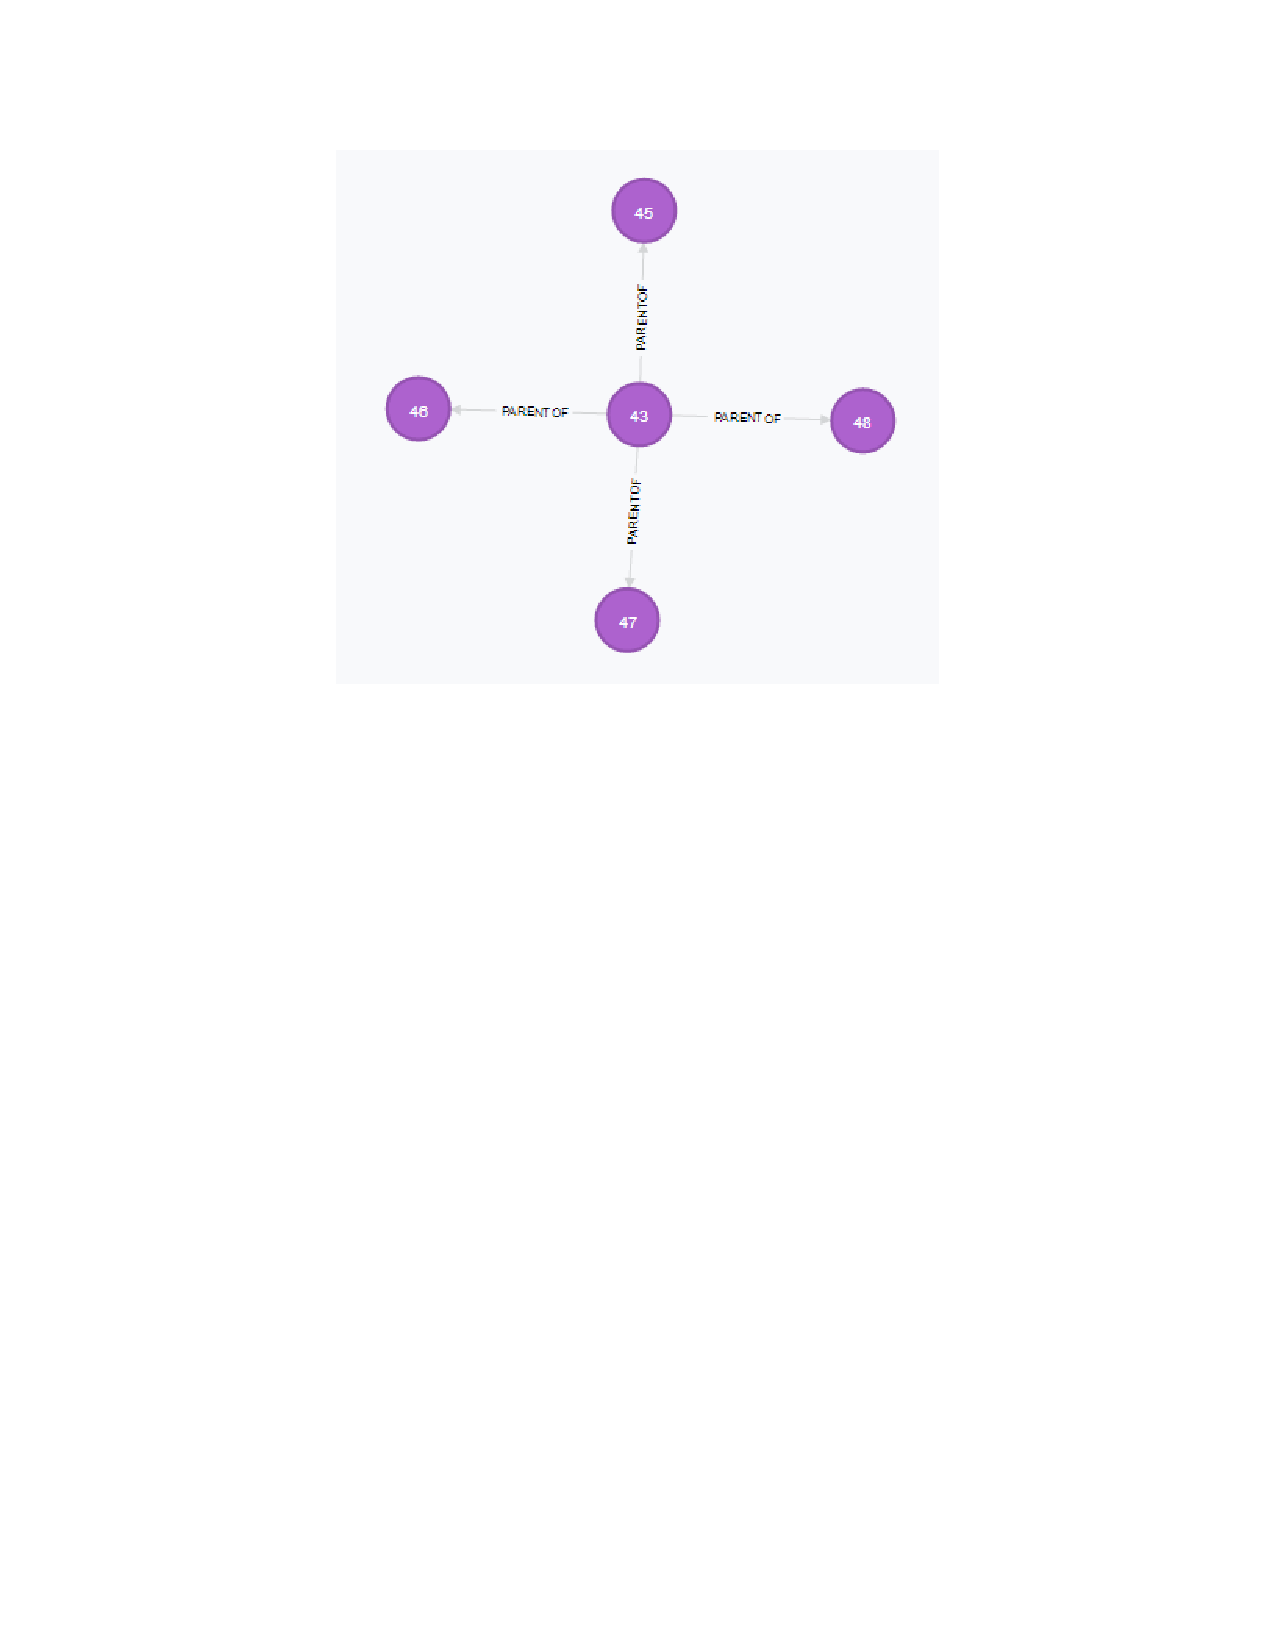
\includegraphics[height=0.68\textwidth]{exampleQuery}
 \caption{Results of Example Query}
 \label{fig:exampleQuery}
\end{figure}

The advantage of a graph database over relational databases relevant to our research was performance. As the dataset grows, relational databases tend to become highly inefficient, as the entire dataset must be searched in response to each query. In graph databases, however, the portion of the dataset that must be searched is limited because the query will only search along an available path connected by relationships. Therefore, this structure allows queries to remain efficient~\cite{GraphDatabases:2013}.





%The experiment described here use two problems: 3SAT and ONESMAX. Solutions to these problems are naturally expressed as bitstrings, and they span a broad range of difficulties. ONESMAX is trivial to solve, and 3SAT problems range from easy to extraordinarily difficult. The specifics of their properties, as well as their implementation in our system are described below.

%\subsection{The 3SAT Boolean Satisfiability Problem}
%\label{sec:3sat}
%The Boolean Satisfiability Problem, or SAT is an NP-Complete problem where the goal is to find an assignment of values to boolean variables that satisfy each clause in a set of clauses. In 3SAT each clause consists of 3 terms each of which is a variable or a negated variable. A clause is said to be satisfied if at least on of its terms is true. A potential solution consists of an assignment of either true or false to each of the variables. A solution that solves the problem, will be one that satisfies every clause. 

%For example, consider SAT problem E, which has four variables, $x_{1}, x_{2}, x_{3}, x_{4}$ and the the two conjoined clauses $(x_{1} \vee x_{2} \vee x_{3}) \wedge (\neg x_{1} \vee x_{3} \vee \neg x_{4})$. For this problem to be solved, both clauses must be satisfied. For a clause to be satisfied, at least one of its terms must be true. So, for example, say we have a potential solution A, which consists of the variable settings $x_{1} =$ true, $x_{2} =$ false, $x_{3} =$ false, and $x_{4} =$ false. The first clause would be satisfied because it contains $x_{1}$, which is true. The second clause would also be satisfied, because $x_{4}$ is false, but the variable in the clause is negated, so $\neg x_{4}$ returns true, which satisfies the clause. As both clauses are satisfied, this assignment solves the problem.	

%Here individuals are represented by bitstrings whose length is equal to the number of variables in the SAT problem~\cite{Gottlieb:2002:EAS:638548.638550}. Each bit represents whether or not a given variable is assigned true or false. The fitness of a potential solution is determined by dividing the number of clauses satisfied by the number of total clauses. Therefore, fitness is always in the range [0,1], representing the proportion of clauses solved. It is important to note that two individuals may have the same fitness but satisfy different clauses.

%In this paper we use three different 3SAT problems as described in Section~\ref{sec:experiments}.

%\subsection{ONESMAX Problem}
%\label{sec:ONESMAX}

%The ONESMAX problem is a simple problem where the goal is to maximize the number of ones in a bitstring~\cite{Alba:2008}. Different ONESMAX problems consist of different lengths of bitstrings. The fitness is simply the number of 1s in the bitstring divided by the length of the bitstring. In this paper, the only ONESMAX problem is one of size 100.





\section{Experimental Setup} 
\label{sec:experiments}

This section explains the details of the configurations used for this research. Subsection \ref{sec:GPSetup} covers setup of the genetic programming algorithm, and Subsection \ref{sec:Neo4jSetup} discusses setup of the graph database Neo4j.

\subsection{Genetic Programming Setup}
\label{sec:GPSetup}

In all of the runs, the configurations remained consistent, with the exception of population size. In the several runs that were performed, the population size was either 1,000, or 10,000. The target function was as follows:
\[
    \sin(x)
\]
where the value of the variable $x$ ranged from 0 to 6.2, increasing by steps of 0.1. The constants allowed were doubles that ranged between -5 and 5, and $x$ was the sole variable. The operations allowed in order to achieve an optimal solution to the target were the binary operations: addition, subtraction, multiplication, and division. Since division is undefined when the denominator is equal to zero, we implemented protected division. In our protected division, if the denominator equals zero, then regardless of the numerator value the output will be one. The reason we chose the output one for protected division is so there would not be a discontinuity in the function $x/x$ when $x = 0$. Therefore, when evolving $x/x$ in a individual we will continue to obtain the value one.

In our system, individuals contain two items: a function called the tree, and the tree's fitness. trees are represented in prefix notation by arrays containing variables, constants, and operators. Prefix notation is a way to write  a function that places the operator before its arguments. For example, a tree of the function $x + (x * 4)$ would be represented by the following array: [+,~x,~*,~x,~4]. The tree's fitness is the sum of the absolute error between the target function and the tree at all predetermined variable values. The absolute error is  the measured value of a quantity $x_{0}$ and its actual value $x$, given by the equation $\Delta x=x_{0}-x$.

After the tree's fitness is computed, we add a constant to the fitness as a means to penalize particularly large trees. This encourages trees to not become excessively large, and is commonly referred to in genetic programming as bloat control. We selected this constant to be a hundredth of the tree size. This implementation of bloat control is relatively weak in the beginning of a run where trees usually have larger fitnesses (therefore not penalizing them unreasonably), but has a significant impact later in the run, where trees should have smaller fitnesses.

To create the initial population, we implemented an algorithm called PTC2~\cite{Luke2013Metaheuristics}. The PTC2 algorithm creates trees by randomly adding operators to an array (leaving blank indices where appropriate for arguments) until a specified length is reached. The blank indices are then filled by leaves (variables and constants). Leaves consist of 63\% variables and 37\% constants.

In order to selection those individuals which will produce the next generation, we  implemented tournament selection. In our tournament, two individuals are selected from the entire generation. The individual with the best fitness of the two selected is chosen to propagate its code in some capacity on to the next generation. This process repeats for the creation of every individual in the next generation.

As discussed previously, individuals may pass on their code by three different means: crossover, mutation, and reproduction. Crossover makes up 90\% of all transformations, mutation 1\%, and reproduction accounts for the remainder. Reproduction is relatively straightforward. The individual which wins the tournament is simply copied on to the next generation. A variation on reproduction is elitism, where an individual is copied to the next generation by merit of it fitness. In other words, within a generation, 1\% of individuals with the best fitness skip tournament and are simply copied over to the next generation. Mutation and crossover are more complex processes, and will be covered in the following paragraphs.

Mutation begins in a similar manner to reproduction. Two individuals are selected from the population to enter the tournament, and the winner is chosen for mutation. However, rather than simply copying this individual on to the next generation, a random index from within the tree is selected. If the index is a operator, the subtree starting at that operator is removed. A subtree is a section of a tree that is itself a valid tree. Otherwise, if the index is a leaf, the index is removed. In both cases, the removed index or indices are replaced by a new subtree generated by PTC2 that is at most half the size of the original tree. This limitation has been put in place to help in controlling bloat.

Crossover differs from the previous transformations in that it makes two calls to the tournament in order to receive two individuals to produce a single child individual in the next generation. The first tournament results in a root parent. Within this parent, similar to mutation, a random index is chosen. If the index is an operator, the subtree is removed, otherwise only the index is removed. The removed index or indices are then replaced by a subtree randomly selected from the individual that won the second tournament.

\subsection{Neo4j Setup}
\label{sec:Neo4jSetup}

In Neo4j, we set nodes to be individuals and defined their ancestry as relationships. Inside each node, we inserted several attributes belonging to an individual. In addition to the tree and fitness, all nodes also include the penalized fitness, the generation number, the transformation type, the run id (used to differentiate between different runs), and a unique id (used for identifying the specific node). For individuals produced by either crossover or mutation, the ``cut point'' (the index at which the root parent was altered by a transformation) is also included as an attribute. These attributes are summarized in Table~\ref{tab:individualAttributes}.
\begin{table}[tb]
\begin{center}
\resizebox{15cm}{!}{
\begin{tabular}{|l|r|r|r|r|r|r|r|r|}
    \hline
    \multicolumn{9}{|c|}{\textbf{Individual Attributes}} \\
    \hline
    \textbf{Transformation} & \textbf{Tree} & \textbf{Fitness} & \textbf{Penalized Fitness} & \textbf{Generation Number} & \textbf{Transformation Type} & \textbf{Run ID} & \textbf{Unique ID} & \textbf{Cut Point} \\ \hline
    Elitism & X & X & X & X & X & X & X & \\
    Reproduction & X & X & X & X & X & X & X & \\
    Mutation & X & X & X & X & X & X & X & X \\
    Crossover & X & X & X & X & X & X & X & X \\
    \hline
\end{tabular}
}
\caption{Chart summarizing attributes that are recorded for individuals produced by each transformation type.}
\label{tab:individualAttributes}
\end{center}
\end{table}

Each individual has a relation to its parent (or parents in the case of crossover). To distinguish between each type of transformation, different types of relationships are used. These relationships are demonstrated in Table~\ref{tab:relationshipTypes}.
\begin{table}[tb]
\begin{center}
\begin{tabular}{|l|l|}
    \hline
    \multicolumn{2}{|c|}{\textbf{Relationship Types}} \\
    \hline
    Reproduction & PARENTOF \\
    Elitism & ELITISM \\
    Mutation & MUTANTOF \\
    Crossover Root & ROOT\textunderscore XOOF \\
    Crossover Non-Root & NONROOT\textunderscore XOOF \\
    \hline
\end{tabular}
\caption{On the left are the various transformation types and on the right are the relationship types assigned to each in the Neo4j database. Notice that crossovers have two relations because two parents were selected in tournament.}
\label{tab:relationshipTypes}
\end{center}
\end{table}





%This section will explain the specifics of the various configurations that were used for this research. For our runs, we used two different kinds of worlds, 2D worlds and 3D worlds. We also had two kinds of problems, the SAT problem, and the ONESMAX problem. This means that there were essentially four main groups of runs, as both kinds of worlds were run with both kinds of problems.

%We tested three different kinds of SAT problems, see Table~\ref{tab:problemFiles}, and the length 100 ONESMAX problem. The SAT problems were selected from various databases and the difficulty assigned to them is taken from~\cite{ellgren:2011}. 

%\begin{table}[tb]
%\begin{center}
%\begin{tabular}{lccl}
%	\textbf{File Name} & \textbf{\# Variables} & \textbf{\# Clauses} & \textbf{Difficulty} \\ \hline
%	uf50-0456.cnf & 50 & 218 & Easy \\
%	uf75-015.cnf & 75 & 325 & Medium \\
%	uf100-0193.cnf & 100 & 430 & Medium \\
%\end{tabular}
%\caption{The 3SAT problems we ran. The difficulties are as reported in~\cite{ellgren:2011}.}
%\label{tab:problemFiles}
%\end{center}
%\end{table}

%We selected three different world sizes for both the 2D and 3D worlds. We used world sizes that were squares or near cubes while also picking sizes that had similar numbers of total locations. The world sizes, as well as how many locations each had are described in Table~\ref{tab:worldsizes}.

%\begin{table}[tb]
%\begin{center}
%\begin{tabular}{lccl}
%	\textbf{2D World Size} & \textbf{\# of locations} \\ \hline
%	10 by 10 & 100 \\
%	15 by 15 & 225 \\
%	24 by 24 & 576 \\
%	27 by 27 & 729 \\
%\end{tabular}
%\begin{tabular}{lccl}
%	\textbf{3D World Size} & \textbf{\# of locations} \\ \hline
%	4 by 5 by 5 & 100 \\
%	6 by 6 by 6 & 216 \\
%	8 by 8 by 9 & 576 \\
%	9 by 9 by 9 & 729 \\
%\end{tabular}
%\caption{The various world sizes we tested.}
%\label{tab:worldsizes}
%\end{center}
%\end{table}

%Sometimes a specific set of parameters works very well for a certain problem and world type, but works poorly for another. So we explored a variety of parameters for both worlds in an attempt to reduce parameter bias. We selected a number of parameters to vary from run to run so that we could compare ``good setups'' to other ``good setups''. The parameters we chose to vary and how we varied them are explained in the Table~\ref{tab:parameters} and were chosen based on our experience with previous experiments with LandscapeEC.

%\begin{table}[tb]
%\begin{center}
%\begin{tabular}{|l|l|}
%	\hline
%	\multicolumn{2}{|c|}{Parameters} \\
%	\hline
%	Average Mutations & 1, 2 \\
%	Carrying Capacity & 15, 30 \\
%	Reproduction Rate & 1, 3 \\
%	Starting Population & Origin, Corners \\
%	\hline
%\end{tabular}
%\caption{On the left are the various parameters we varied and to their right are the different values we assigned them.}
%\label{tab:parameters}
%\end{center}
%\end{table}

%There were 512 different problem and parameter settings. Each run with a specific set of parameters was run 30 times which means there was a total of 15360 runs.





\section{Results} \label{sec:results}

\begin{figure}[tb]
 \centering
 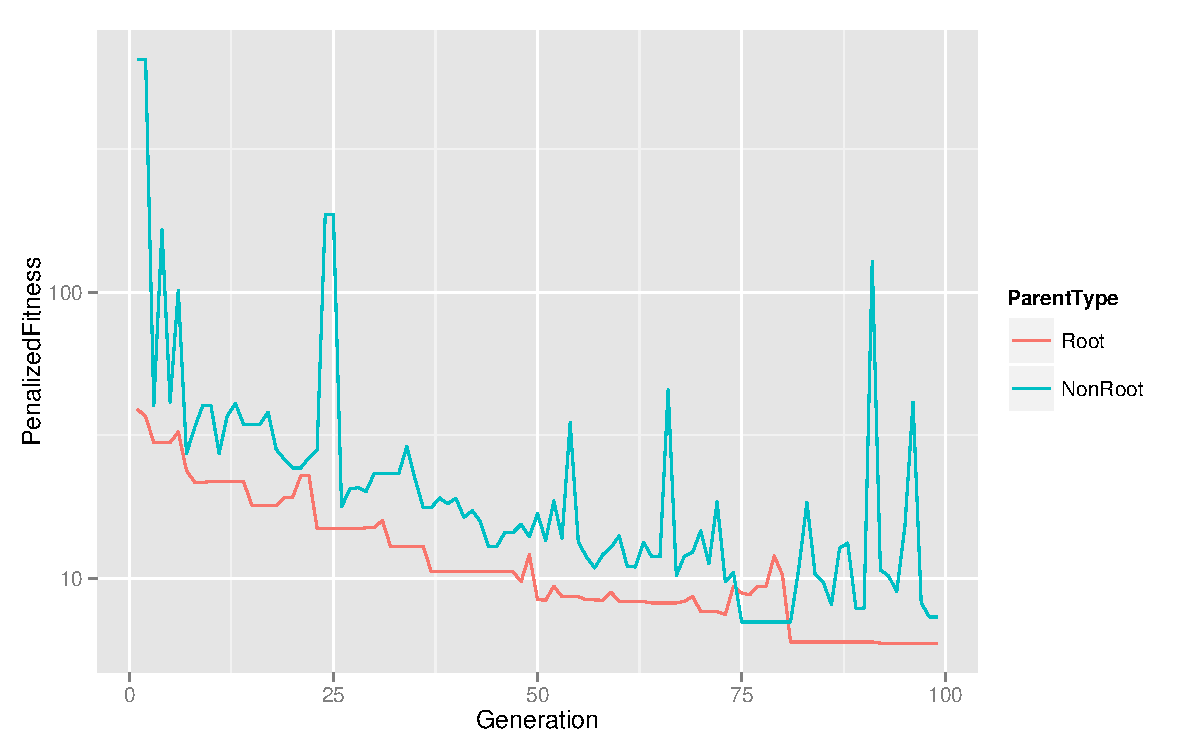
\includegraphics[height=0.68\textwidth]{Root_vs_nonroot_line_fitnesses}
 \caption{Root Versus Non-Root Fitness in Ancestry of Best Tree from Final Generation of a 1K Run}
 \label{fig:rootVsNonrootFitness}
\end{figure}



%Table~\ref{tab:parameters} lists the most successful parameter values of those we explored , as well as the success rates and median evaluations used for those parameters. Asterisks indicate parameter settings whose values didn't make a statistically significant difference for that configuration. Figure~\ref{fig:evalPlots} shows the distribution of completed evaluations for the best parameter values.

%\begin{table}[tb]
%\begin{center}
%\begin{tabular}{|l||l|l||l|l|}
%	\hline
%	& \multicolumn{2}{|c||}{3SAT} & \multicolumn{2}{|c|}{ONESMAX} \\
%	\hline
%	& \textbf{2D} & \textbf{3D} & \textbf{2D} & \textbf{3D} \\ \hline
%	World Size & 24x24,27x27 & 8x8x9, 9x9x9 & * & 4x4x5 \\
%	Starting Locations & Corners & Corners & Origin & * \\
%	Carrying Capacity & * & * &	* & 15 \\
%	Reproduction Rate & * & * & 1 & * \\
%	Average Mutations & * & * & 1 & * \\
%	Success Rate &	69\% & * 64\% & 100\% & 100\% \\
%	Median \# of Evals & 3,958,000 & 4,709,000 & 49,890 & 42,950 \\
%	\hline
%\end{tabular}
%\caption{This table diagrams the best configurations and their success rates and median number of evaluations.}
%\label{tab:results}
%\end{center}
%\end{table}

%\begin{figure}[tb]

% \centering
% \includegraphics[height=0.68\textwidth]{CompletedEvalsAll.pdf}
% \caption{A box-and-whisker plot of the number of completed evaluations for each version. Note the log-scale on the y-axis.}
% \label{fig:evalPlots}

%\end{figure}

%On the 3SAT problems 2D worlds did significantly better than 3D worlds; they succeeded more times and faster. A Kruskal-Wallis test confirms that the difference is significant with a p-value of 2.327e-8. Interestingly for both 2D worlds and 3D worlds large world sizes and starting in the corners were important parameters, while the other three parameters were negligible in effect. 

%In an unexpected twist, 3D worlds did solved the ONESMAX problem faster than 2D worlds, although they both had the same success rate of 100\%. Also, where before the important parameters were the same when solving 3SAT. The difference in speed was confirmed to be statistically significant with a p-value of 2.2e-16. 2D and 3D worlds have completely different parameters that are important in ONESMAX. 2D worlds found reproduction rate, starting locations, and average mutations to be important, while 3D worlds only found world size and carrying capacity to be important.





\section{Conclusions} \label{sec:conclusion}

A critical point is that graph databases like Neo4j don't make anything possible that was once impossible; they instead make these things vastly simpler and allow open-ended exploration. Each of the queries and questions we've discussed could be handled by, for example, special purpose code added to the evolutionary system to specifically capture that specific information. Many, if not most, of these have no doubt been addressed in a piecemeal fashion by previous research. We observed (GECCO 99 paper) nearly 15 years ago, for example, that root parent lineages were significant, and that these lineages quickly coalesced into a shared common ancestor, but that was using a specialized custom system to track that data, and there has been limited follow-up, by us or others, since then. We suspect a significant reason for the lack of similar work is simply the effort required to collect and analyze the substantial amount of data this entails, and the lack of good tools to simplify that process.





%We suspect that the reason why 2D worlds do better than 3D worlds when solving 3SAT is a matter of distance and diversity. 3SAT problems tend to to have a large number of local optima that EC systems can fall into. Because of this, maintaining diversity is key. This may suggest why corners are so important, there needs to be more than one starting population because there's a strong chance that each population is very different from another. However, diversity isn't maintained in 3D systems due to the distance between starting locations. In the largest 3D world, the distance between a starting location and another starting location was as small as nine locations. Meanwhile, in a 2D world, the distance between starting locations was a factor of three larger, with the the largest world being 27 across. What is happening is a local optima is found, which can spread much more quickly in a 3D world than in a 2D world due to the smaller distances between any two locations in the 3D worlds. This compromises diversity and caused 2D worlds to perform better in our runs.

%Meanwhile, the ONESMAX problems are completely different. They have no local optima to fall for, so the system has a different approach to solving them. In 3D worlds, smaller potential populations are better because you want the number of new individuals to be minimized, to a point. The problem will often be solved so quickly that new individuals don't have time to ``mature'' and contribute to solving the problem.

%In 2D worlds, world size doesn't matter as much, because the world almost never fills before the problem is solved. Origin is important because the problem is solved so fast that corners never have time to spread out fast enough to interact meaningfully, so starting in one spot saves evaluations.       

%Overall, although 3D worlds didn't solve 3SAT faster, it illustrated the importance of distance in cEA systems. Having a large distance between starting locations is good for maintaining diversity, while if maintaining diversity isn't an issue, then more starting locations are better. A potential route of future research is to decrease the number of connections between locations and try to spread them more thinly. This is essentially trying to do the opposite of what 3D worlds do, where there is an increased number of connections as well as shorter distances between locations.





\section*{Acknowledgements}





%Many thanks to Lucas Ellgren for his feedback and for the use of several diagrams.

%This work was supported in part by the Morris Academic Partners program at the University of Minnesota, Morris.

\bibliographystyle{acm}
\bibliography{MICS_2014}

\end{document}
